\begin{frame}
    \subsection{Operations}
    \frametitle{B-Tree Operations}
    \begin{columns}
        \begin{column}{\textlecolumn}
            \begin{block}{}
                \begin{itemize}
                    \item For these operations, we will assume that the whole B-Tree is loaded into main memory.
                    \item We have to asume this since the main usage of the B-Tree is oriented to secondary storage.
                    \item Generally, only the \emph{Root} and node to operate, if available, will be always available in memory.
                    \item But if we need any other node, we will have to read into our secondary memory and fetch it's data.
                    \item This process takes more time than the general data fetch from main memory.
                    \item So, the fewer times we do this process the better.
                \end{itemize}
            \end{block}
        \end{column}
        \begin{column}{\textricolumn}
        \end{column}
    \end{columns}
    \begin{figure}[h!]
        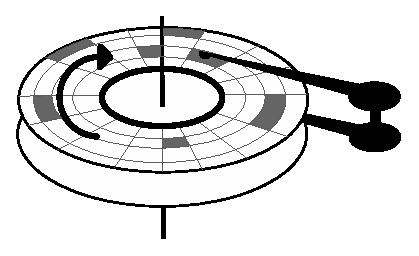
\includegraphics[width=0.5\textwidth]{resources/made/external_storage_wblocks.eps}
        \caption{External storage with the sectors to access highlighted}
    \end{figure}
\end{frame}
